\documentclass[final,14pt,t]{beamer}
%\documentclass[final,17pt,t]{beamer}
\mode<presentation>{\usetheme{Purdue}}

\usepackage{natbib,url}
\usepackage{multicol}
\usepackage{geometry}
\usepackage{multirow}
\usepackage{rotating}
\usepackage{wrapfig}

\usepackage{tikz}
\usetikzlibrary{shapes,arrows}
\usepackage{graphicx}
\usepackage{tikz-dependency}
\usepackage{natbib}
\usepackage{url}
%\usepackage{gb4e}
\usepackage{amsmath}
\DeclareMathOperator*{\argmax}{arg\,max}
\DeclareMathOperator*{\argmin}{arg\,min}
% MD: This threw an odd error for me:
%\usepackage{tikz-qtree}
\usepackage[framemethod=tikz]{mdframed}

\newcommand{\myboxedtext}[2][rectangle,draw,rounded corners]{%
            \tikz[baseline=-0.6ex] \node [#1,rounded corners]{#2};}%

\usepackage{enumerate}
\usepackage{color}
\usepackage{xcolor}
\usepackage{caption}
\setbeamerfont{caption}{size=\normalsize}

%\definecolor{light-gray}{gray}{0.9}
%\definecolor{forestgreen}{rgb}{0.13, 0.55, 0.13}
%\definecolor{carnelian}{rgb}{0.7, 0.11, 0.11}
%\definecolor{darkblue}{rgb}{0.0, 0.0, 0.55}
%\definecolor{darkgreen}{rgb}{0.0, 0.2, 0.13}
%\definecolor{persimmon}{rgb}{0.93, 0.35, 0.0}

\usepackage[size=custom,width=120,height=90,scale=1]{beamerposter}
\usepackage{gb4e}

\title[]{Annotating Picture Description Task Responses for Content Analysis}
\author[]{Levi King \& Markus Dickinson}
\institute[]{Indiana University}
\date[]{5 June 2018}
\newcommand{\myimg}{
  \framebox{
   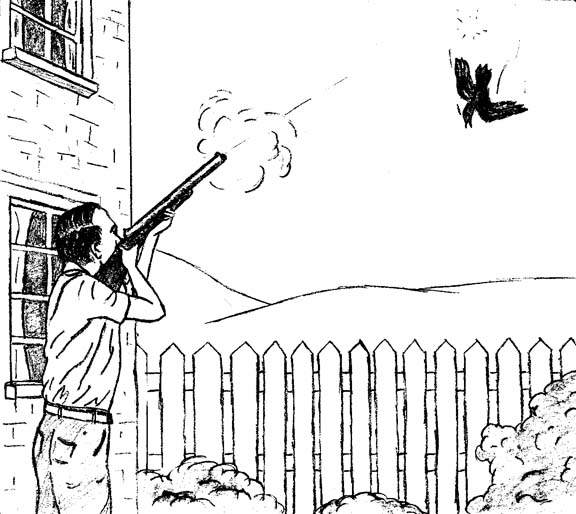
\includegraphics[width=.95\textwidth]{../figures/exampleprompt2.jpg}}}
\setbeamertemplate{caption}[numbered]
\setbeamertemplate{itemize/enumerate body begin}{\normalsize}
\setbeamertemplate{itemize/enumerate subbody begin}{\normalsize}
\setbeamertemplate{itemize/enumerate subsubbody begin}{\normalsize}

\begin{document}
\begin{frame}{}
  \begin{columns}[t]
    \begin{column}{.33\linewidth}
\begin{minipage}[t][\textheight]{\linewidth} 

\vspace{-1.7em}
\begin{block}{Overview}
\begin{center}
\begin{minipage}{.85\textwidth}

\vspace{.6em}
  \begin{itemize}
    \itemsep1em
  \item{\textbf{Semantic Analysis of Image-based Learner Sentences (SAILS) Corpus}
   \medskip
	\begin{itemize}
   \item 13,533 picture description task (PDT) responses
     %from native (NS) \& non-native speakers (NNS)
   \item Both native (NS) \& non-native speakers (NNS)
   \item Annotated for five binary features
      \end{itemize}
    }
\end{itemize}

\vspace{.6em}

  \begin{itemize}
    \itemsep1em
  \item{\textbf{Goal:} Evaluate content of NNS sentences 
      \begin{itemize}
      \item Compare to gold standard (GS) of NS sentences
      \end{itemize}
    }
\end{itemize}

\vspace{.6em}

  \begin{itemize}
    \itemsep1em
  \item{\textbf{Need:}  Adequate data, appropriately constrained
        \begin{itemize}
      \item Large set of PDT responses % from NS and NNS participants
      \item Varied task prompts \& participant demographics % allowing for study of variability
      \item Annotation for content analysis
      \end{itemize}
    }
\end{itemize}

\end{minipage}
\end{center}
\end{block}



\begin{block}{Picture Description Task}
\begin{center}
\begin{minipage}{.85\textwidth}

  \vspace{1em}
  \begin{itemize}
  \item{PDT elicits natural productions but constrains form \& content}
  \vspace{.6em}
  \item{60 \textbf{items}: 30 images $x$ 2 prompts}
  \vspace{.6em}
    % \begin{itemize}
    % \item 30 images
    % \begin{itemize}
    % 	\item simple vector graphics
    %     	\item 10 transitive, 10 intransitive, 10 ditransitive actions
    %     \end{itemize}
    % \item 2 prompts:
    % 	\begin{itemize}
    %     		\item \textbf{targeted}: \textit{What is $<$the subject$>$ doing?}
    %     		\item \textbf{untargeted}: \textit{What is happening?}
    %     	\end{itemize}
    %     \end{itemize}
  \end{itemize}
  \begin{tabular}{cc}
  \vspace{1em}
    \begin{minipage}{.45\textwidth}
      \begin{center}
        \vspace{1ex}
        30 images
      \end{center}
        \vspace{-1ex}
    \begin{itemize}
    \item Simple vector graphics
    \item 10 intransitive, 10 trans, 10 ditrans
    \end{itemize}
    \end{minipage}
    & 
    \begin{minipage}{.51\textwidth}
      \begin{center}
        \vspace{1ex}
        2 prompts
      \end{center}
        \vspace{-1ex}
    \begin{itemize}
    \item \textbf{Targeted}: \textit{What is $<$the subject$>$ doing?}
    \item \textbf{Untargeted}: \textit{What is happening?}
    \end{itemize}
    \end{minipage}
    \\
  \end{tabular}

	\bigskip
\setlength{\fboxsep}{3pt}
\setlength{\fboxrule}{0pt}
\begin{table}[htb!]
\begin{center}
\begin{tabular}{|c|c|c|}
\hline
Intransitive & Transitive & Ditransitive \\
\hline
{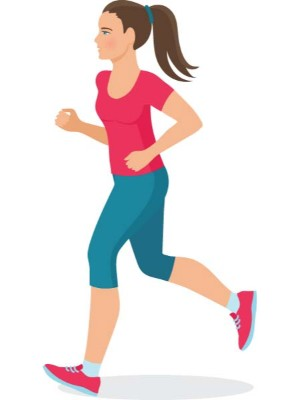
\includegraphics[width=0.29\columnwidth]{../figures/I30.jpg}} & {
\includegraphics[width=0.3\columnwidth]{../figures/I29.jpg}} & {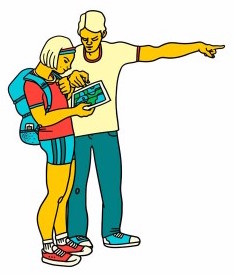
\includegraphics[width=0.3\columnwidth]{../figures/I28.jpg}} \\
What is the woman doing? & What is the woman doing? & What is the man doing? \\
\hline
%\hline
%{
\includegraphics[width=0.29\columnwidth]{../figures/I20.jpg}} & {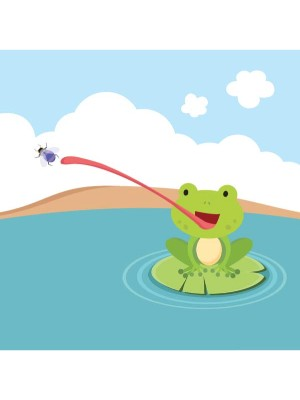
\includegraphics[width=0.3\columnwidth]{../figures/I16.jpg}} & {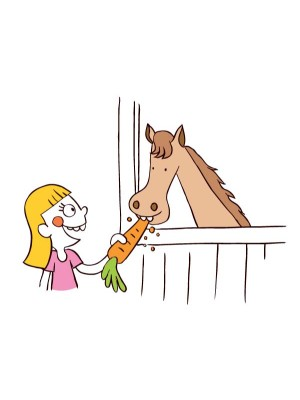
\includegraphics[width=0.3\columnwidth]{../figures/I17.jpg}} \\
%What is the girl doing? & What is the frog doing? & What is the girl doing? \\
%\hline
\end{tabular}
\medskip
\caption{\label{tab:example-pdt-items} Example PDT images with their \textbf{targeted} questions.} % In the \textbf{untargeted} form, the question for each is \textit{What is happening?}} %From left to right, the examples represent two intransitive, transitive and ditransitive items.}
\end{center}
\end{table}

Administered as online survey (SurveyMonkey.com)

%\begin{center}
%  \textit{PDT Instructions}
%  % Focus on main action; Respond with complete sentence
%\end{center}
%\begin{center}
%  \begin{minipage}{.4\textwidth}
%    \begin{itemize}
%    \item Focus on the main action
%    \item Respond in a complete sentence
%    \end{itemize}
%  \end{minipage}
%\end{center}
\vspace{.6em}
  \textit{PDT Instructions}
  % Focus on main action; Respond with complete sentence
    \begin{itemize}
    \item Focus on the main action
    \item Respond in a complete sentence
    \end{itemize}

\vspace{.6em}
	% \item PDT Instructions: 
        %   %Focus on main action; Respond with complete sentence
	% \begin{itemize}
	% 	\item Focus on the main action
	% 	\item Respond in a complete sentence
	% \end{itemize}
Multiple versions
	\begin{itemize}
		\item Most participants completed 30 items
		\item Roughly equal number of targeted \& untargeted responses % collected per image
		\item NNSs provide one response per item
		\item NSs provide two non-identical responses per item (more robust GS)
		% \begin{itemize}
		% 	\item[$\Rightarrow$] 
                %           %Intended to increase variety of NS responses for 
                %           More robust GS
		% \end{itemize}
	\end{itemize}

%\begin{center}
%  Task administered as online survey (SurveyMonkey.com)
%\end{center}

\end{minipage}
\end{center}
\vspace{-.5em}
\end{block}

\begin{block}{Participants}

\begin{center}
\begin{minipage}{.85\textwidth}
\begin{center}
499 total participants
\end{center}
	\begin{itemize}
		\item 141 NNSs: students in intermediate \& advanced ESL writing courses at IU
		\begin{itemize}
		\vspace{.3em}
%			\item Recruited from intermediate \& advanced English as a Second Language writing courses at Indiana University
			%\item From intermediate \& advanced ESL writing courses at IU
			%\item Performed task in computer lab with researchers present
			\item L1s: 125 Chinese (90\%), 4 Korean, 3 Burmese, 2 Hindi; 1 each: Arabic, Indonesian, German, Gujarati, Spanish, Thai, Vietnamese
		\end{itemize}
		\vspace{.8em}
		\item 358 NSs
		\begin{itemize}
			\vspace{.4em}
			%\item All NSs performed task remotely
			\item 29 Familiar Native Speakers (FNSs)
			\begin{itemize}
				\item Relatives or friends of researchers (assumedly higher quality)
%				\item Responses are assumed to be high quality
			\end{itemize}
			\vspace{.4em}
			\item 329 Crowdsourced Native Speakers (CNSs)
			\begin{itemize}
				\item Responses purchased via SurveyMonkey (assumedly lower quality)
				%\item Limited by SurveyMonkey to only 15 items per participant
%				\item Responses are assumed to be lower quality
			\end{itemize}
		\end{itemize}
	\end{itemize}
	\vspace{1.3em}
\end{minipage}
\end{center}
\vspace{-.5em}
\end{block}
\end{minipage}
\end{column}

\begin{column}{.33\linewidth}
\begin{minipage}[t][\textheight]{\linewidth} 

\vspace{-1.7em}

\begin{block}{Responses}
\begin{center}
\begin{minipage}{.85\textwidth}

%The SAILS Corpus contains a total of 13,533 PDT responses

\begin{center}
  \textbf{Response Counts}
\end{center}

%\vspace{.1em}
\begin{table}[htb!]
\begin{center}
\setlength{\tabcolsep}{0.65em}
\begin{tabular}{|l||r|r||r|}
\hline
& \multicolumn{3}{|c|}{Response Counts} \\
\hline
 Group & First & Second & Total \\
\hline
\hline
NNS & 4290 & 0 & 4290 \\
\hline
\hline
NS (all) & 4634 & 4609 & 9243 \\ 
\hline
\multicolumn{1}{|r||}{FNS} & 642 & 641 & 1283 \\ 
\hline
\multicolumn{1}{|r||}{CNS} & 3992 & 3968 & 7960 \\
\hline
\hline
Total & 8924 & 4609 & 13,533 \\
\hline
\end{tabular}
\caption{\label{tab:response-counts} First \& second response counts for SAILS Corpus participant groups}
%. Familiar (FNS) and crowdsourced (CNS) are subgroups of NS. NNS participants are not asked to provide a second response.}
\end{center}
\end{table}

\vspace{1.3em}
% In order to examine the level of variation among responses, type to token ratios (TTRs) were calculated on the response level. Capitalization and final punctuation were ignored. We can see that variation increases with item complexity (intransitives $<$ transitives $<$ ditransitives) and that untargeted responses vary more than targeted responses.
% \vspace{.5em}

\begin{center}
  \textbf{Type-Token Ratios (TTRs)}
\end{center}

\begin{table}[h!]
\begin{center}
\setlength{\tabcolsep}{0.65em}
\begin{tabular}{|l||l|l||l|l|}
\hline
 & \multicolumn{2}{|c||}{Targeted} & \multicolumn{2}{|c|}{Untargeted} \\
\hline
 Set & NS & NNS & NS & NNS \\
\hline
\hline
Intransitives & 0.628 & 0.381 & 0.782 & 0.492 \\
\hline
Transitives & 0.752 & 0.655 & 0.859 & 0.779 \\
\hline
Ditransitives & 0.835 & 0.817 & 0.942 & 0.936 \\ 
\hline
\end{tabular}
\caption{\label{tab:ttr} TTRs for \textit{complete responses} (not words), for full corpus}
\end{center}
\end{table}

%\vspace{1em}
% In order to examine the level of variation among responses, type to token ratios (TTRs) were calculated on the response level. 
\begin{itemize}
\item Capitalization \& final punctuation ignored
\vspace{.3em}
\item Variation increases with:
  \begin{itemize}
  \vspace{.3em}
  \item Item complexity (intransitives $<$ transitives $<$ ditransitives)
  \vspace{.3em}
  \item Less targeting (targeted $<$ untargeted)
  \end{itemize}
\end{itemize}
\vspace{1em}

\vspace{1.3em}
% TTRs were also calculated to compare the variability among NSs' first responses versus their second responses. As the TTRs for second responses are considerably higher than those for first responses, asking for two non-identical responses appears to effectively increase the variety of NS responses available for use in a GS.
% \vspace{.5em}

\begin{center}
  \textbf{Type-Token Ratios (TTRs): first vs. second responses (NSs only)}
\end{center}

\begin{table}[hb!]
\begin{center}
\setlength{\tabcolsep}{0.65em}
\begin{tabular}{|l||l|l||l|l|}
\hline
 & \multicolumn{2}{|c||}{Targeted} & \multicolumn{2}{|c|}{Untargeted} \\
\hline
 Set & R1 & R2 & R1 & R2 \\
\hline
\hline
Intransitives & 0.343 & 0.819 & 0.549 & 0.939 \\
\hline
Transitives & 0.509 & 0.895 & 0.682 & 0.926 \\
\hline
Ditransitives & 0.641 & 0.948 & 0.864 & 0.955  \\ 
\hline
\end{tabular}
\caption{\label{tab:ttr1v2} TTRs for complete responses, separated by first (R1) \& second responses (R2)} %. The ratios here are calculated from all NS responses; NNS responses are not included.}
\end{center}
\end{table}

%\vspace{1em}
%TTRs were also calculated to compare the variability among NSs' first responses versus their second responses. As the
\begin{itemize}
\item TTRs for R2s considerably higher than for R1s
  \begin{itemize}
  \vspace{.3em}
  \item[$\Rightarrow$] Asking for two responses increases variety of
    language available for use in GS
  \end{itemize}
\end{itemize}
\vspace{.5em}

\end{minipage}
\end{center}
\vspace{-.5em}
\end{block} 



\begin{block}{Annotation Scheme}
\begin{center}
\begin{minipage}{.85\textwidth}
% Two annotators:
% \begin{itemize}
% 	\item NSs (US English), both with language teaching experience (child \& adult learners).
% 	\item Annotator 1 (A1) annotated the complete corpus, Annotator 2 (A2) annotated development set \& test set, each containing 1 intransitive, 1 transitive, 1 ditransitive.
% \end{itemize}
% \vspace{1em}

\textbf{Initial scheme:} \textit{accurate $+$ native-like} $>$ \textit{accurate $+$ not native-like} $>$ \textit{not accurate})

\vspace{.5em}
\textbf{Final scheme:} five binary features related to accuracy \&
native-likeness: 
\vspace{.6em}
\begin{enumerate}
\item \textbf{Core Event (C)}: Does response capture the core event depicted in image?
%Core events are not pre-defined for annotators but should be obvious given the nature of the images. The response should link an appropriate subject to the event.  In Table~\ref{tab:sample-responses}, \textit{[The woman is] holding a puppy and looks happy} clearly captures the core event, while \textit{She is wear a blue dress} is irrelevant to the event happening.
\vspace{.6em}
\item \textbf{Verifiability (V)}: Does response contain only true \& verifiable info, based on image? 
\begin{itemize}
\vspace{.4em}
\item Inferences allowed only when necessary; e.g., familial relationships of persons in image
\end{itemize}
%For example, in Table~\ref{tab:sample-responses}, \textit{She is wear a blue dress} conveys information that is irrelevant to the core event but is nonetheless recoverable from the image (core event=0, verifiability=1), while \textit{hugging her dog Fluffy that she missed while on vacation} fulfills the core event but also has information that cannot be inferred from the picture (core event=1, verifiability=0).
\vspace{.5em}
\item \textbf{Answerhood (A)}: Does response make a clear attempt to answer the question?
\begin{itemize}
\vspace{.4em}
\item Generally requires a progressive verb
\vspace{.4em}
\item For targeted items: subject of question or appropriate pronoun must be response subject
\end{itemize}
%For example, \textit{The dog is so happy!} is answering a question other than \textit{What is the woman doing?}. 
\vspace{.5em}
\item \textbf{Interpretability (I)}: Does response evoke clear mental image (even if different from PDT)? 
\begin{itemize}
\vspace{.4em}
\item Any required verb arguments must be present \& unambiguous
\end{itemize}
%For example, \textit{She loves her pet} is too vague to generate a clear mental image. No action is specified (unless we force an unlikely reading of \textit{loves} as a dynamic, simple present verb), and we cannot know if the \textit{pet} is a dog, a horse, etc.
\vspace{.5em}
\item \textbf{Grammaticality (G)}: Is response free from errors of spelling \& grammar?  
%In the SAILS responses, this is a relatively straightforward feature to annotate. For example, from Table~\ref{tab:sample-responses}, \textit{She is wear a blue dress} contains an ungrammatical verb form.

\end{enumerate}



\end{minipage}
\end{center}
\vspace{-.5em}
\end{block}



\begin{block}{Annotators}
\begin{center}
\begin{minipage}{.85\textwidth}
Two annotators:
\begin{itemize}
\vspace{.5em}
	\item NSs (US English), both with language teaching experience (child \& adult learners).
	\vspace{.4em}
	\item Annotator 1 (A1): complete corpus
	\vspace{.4em}
    \item Annotator 2 (A2): development \& test sets, each with 1 intransitive, 1 trans, 1 ditrans
\end{itemize}
\end{minipage}
\end{center}
%\vspace{-.5em}
\end{block}

\end{minipage}
\end{column}

\begin{column}{.33\linewidth}
\begin{minipage}[t][\textheight]{\linewidth} 
\vspace{-1.7em}
\begin{block}{Annotation Results}
\begin{center}
\begin{minipage}{.85\textwidth}

%\begin{table}[htb!]
%\begin{center}
%\begin{tabular}{|l|c|c|c|c|c|}
%\hline
%\multicolumn{6}{|c|}{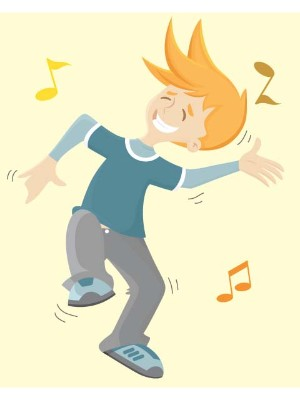
\includegraphics[width=0.29\columnwidth]{../figures/I01.jpg}} \\ 
%\hline
%\textit{What is the boy doing?} (Targeted) & C & V & A & I & G \\
%\hline
%\hline
%eating food. & 0 & 1 & 1 & 1 & 1 \\
%\hline
%eatting. & 0 & 1 & 1 & 1 & 0 \\
%\hline
%The child is about to eat pizza. & 1 & 1 & 0 & 1 & 1 \\
%\hline
%He may get fat eating pizza. & 1 & 0 & 0 & 1 & 1 \\
%\hline
%\hline
%\hline
%\textit{What is happening?} (Untargeted) & C & V & A & I & G \\
%\hline
%\hline
%Child is eating pizza. & 1 & 1 & 1 & 1 & 0 \\
%\hline
%Tommy is eating pizza. & 1 & 0 & 1 & 1 & 1 \\
%\hline
%The boy's eating his favorite food. & 0 & 0 & 1 & 0 & 1 \\
%\hline
%Pizza is this boy's favorite food. & 0 & 0 & 0 & 0 & 1 \\
%\hline
%\end{tabular}
%\caption{\label{tab:devo-transitive} Sample responses from the development set transitive item, shown with adjudicated annotations for the five features: core event (\textit{C}), verifiability (\textit{V}), answerhood (\textit{A}), interpretability (\textit{I}) and grammaticality (\textit{G}).}
%\end{center}
%\end{table}

\begin{center}
  \textbf{Annotation Examples}
\end{center}

\begin{table}[htb!]
\begin{center}
\setlength{\tabcolsep}{0.45em}
\begin{tabular}{|l||l|c|c|c|c|c|}
\hline
\multirow{17}{*}{
\includegraphics[width=0.35\columnwidth]{../figures/I02.jpg}}& \textit{What is the boy doing?} (Targeted) & C & V & A & I & G \\
\cline{2-7}
\cline{2-7}
& eating pizza & 1 & 1 & 1 & 1 & 1 \\
\cline{2-7}
& eating food. & 0 & 1 & 1 & 1 & 1 \\
\cline{2-7}
& eatting. & 0 & 1 & 1 & 1 & 0 \\
\cline{2-7}
& The child is eating pizza. & 1 & 1 & 0 & 1 & 1 \\
\cline{2-7}
& He may get fat eating pizza. & 1 & 0 & 0 & 1 & 1 \\
\cline{2-7}
& The boy is hungry. & 0 & 1 & 0 & 0 & 1 \\
\cline{2-7}
& Pizza is this boy's favorite food. & 0 & 0 & 0 & 0 & 1 \\
\cline{2-7}
& \multicolumn{6}{c|}{} \\
\cline{2-7}
& \textit{What is happening?} (Untargeted) & C & V & A & I & G \\
\cline{2-7}
\cline{2-7}
& The kid's eating pizza & 1 & 1 & 1 & 1 & 1 \\
\cline{2-7}
& Child is eating pizza. & 1 & 1 & 1 & 1 & 0 \\
\cline{2-7}
& Tommy is eating pizza. & 1 & 0 & 1 & 1 & 1 \\
\cline{2-7}
& The boy's eating his favorite food. & 0 & 0 & 1 & 0 & 1 \\
\cline{2-7}
& A youngster anticipates the taste of pizza & 1 & 1 & 0 & 1 & 1 \\
\cline{2-7}
& Pepperoni pizza makes the boy smile & 0 & 0 & 0 & 1 & 1 \\
\cline{2-7}
& He sure is happy. & 0 & 1 & 0 & 1 & 1 \\
\hline
\end{tabular}
\caption{\label{tab:devo-transitive} Sample responses from development transitive item, with adjudicated annotations} % for the five features: core event (\textit{C}), verifiability (\textit{V}), answerhood (\textit{A}), interpretability (\textit{I}) and grammaticality (\textit{G}).}
\end{center}
\end{table}

%\begin{table}[htb!]
%\begin{center}
%\begin{tabular}{|l|c|c|c|c|c|c|l|c|c|c|c|c|}
%\hline
%\multicolumn{13}{|c|}{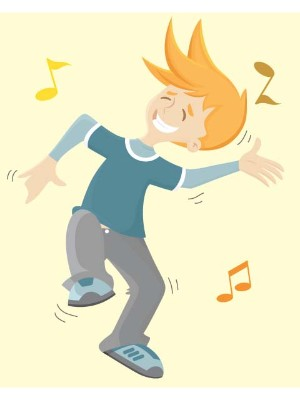
\includegraphics[width=0.29\columnwidth]{../figures/I01.jpg}} \\ 
%\hline
%\textit{What is the boy doing?} & C & V & A & I & G && \textit{What is happening?} & C & V & A & I & G \\
%\hline
%\hline
%eating food. & 0 & 1 & 1 & 1 & 1 && Child is eating pizza. & 1 & 1 & 1 & 1 & 0 \\
%\hline
%eatting. & 0 & 1 & 1 & 1 & 0 && Tommy is eating pizza. & 1 & 0 & 1 & 1 & 1 \\
%\hline
%The child is about to eat pizza. & 1 & 1 & 0 & 1 & 1 && The boy's eating his favorite food. & 0 & 0 & 1 & 0 & 1 \\
%\hline
%He may get fat eating pizza. & 1 & 0 & 0 & 1 & 1 && Pizza is this boy's favorite food. & 0 & 0 & 0 & 0 & 1 \\
%\hline
%\end{tabular}
%\caption{\label{tab:devo-transitive} Targeted and untargeted sample responses shown with adjudicated annotations for the development set transitive item (see Table~\ref{tab:example-pdt-items}).}
%\end{center}
%\end{table}

\vspace{1em}

\begin{center}
  \bf Inter-Annotator Agreement
\end{center}
\vspace{-.5em}
% Using test set items from Table~\ref{tab:example-pdt-items}, we calculated inter-annotator agreement for each feature, for targeted vs. untargeted items, and for the three verb types.
% %, as shown in Table~\ref{tab:agreement}. 
%\vspace{1em}
\begin{table}[htb!]
\begin{center}
% MD: this gives a bit more spacing between columns:
\setlength{\tabcolsep}{0.65em}
\begin{tabular}{|l|l|l|l|l|l||l|l||l|}
\hline
& Set	& Total	& A1Yes & A2Yes & AvgYes & Chance & Agree & Kappa \\
\hline
\hline
\multirow{3}{*}{Verb Type}& Intransitive & 2155 & 0.863 & 0.855 & 0.859 & 0.758 & 0.978 & 0.910 \\
\cline{2-9}
& Transitive & 2155 & 0.780 & 0.774 & 0.777 & 0.653 & 0.949 & 0.853 \\
\cline{2-9}
& Ditransitive & 2155 & 0.812 & 0.786 & 0.799 & 0.678 & 0.924 & 0.764 \\ 
\hline
\hline
\multirow{2}{*}{Prompt} & Targeted & 3390 & 0.829 & 0.818 & 0.824 & 0.709 & 0.949 & 0.823 \\
\cline{2-9}
& Untargeted & 3075 & 0.806 & 0.790 & 0.798 & 0.678 & 0.952 & 0.872 \\
\hline
\hline
\multirow{5}{*}{Feature} & Core Event & 1293 & 0.733 & 0.717 & 0.725 & 0.601 & 0.923 & 0.808 \\
\cline{2-9}
& Verifiability & 1293 & 0.845 & 0.817 & 0.831 & 0.719 & 0.968 & 0.884 \\
\cline{2-9}
& Answerhood & 1293 & 0.834 & 0.831 & 0.833 & 0.721 & 0.982 & 0.936 \\
\cline{2-9}
& Interpretability & 1293 & 0.818 & 0.787 & 0.802 & 0.682 & 0.919 & 0.744 \\
\cline{2-9}
& Grammaticality & 1293 & 0.861 & 0.872 & 0.866 & 0.768 & 0.960 & 0.827 \\
\hline
\end{tabular}
\caption{\label{tab:agreement} Agreement scores broken down by different properties of test set}
%: total annotations (\textit{Total}), \textit{yes} annotations for Annotator 1 and 2 (\textit{A1Yes}, \textit{A2Yes}), average \textit{yes} annotations (\textit{AvgYes}), total expected chance agreement for \textit{yes}es and \textit{no}s (\textit{Chance}), actual raw agreement (\textit{Agree}) and Cohen's kappa (\textit{Kappa}).}
\end{center}
\end{table}
\vspace{1em}

\begin{center}
  Observations from Table~\ref{tab:agreement}
\end{center}
\begin{itemize}
	\vspace{.2em}
	\item Average \textit{yes} rates (\textit{AvgYes}) show all features skew toward \textit{yes} annotations
          \begin{itemize}
          \vspace{.2em}
          \item Cohen's kappa needed as measure of inter-annotator agreement
          \end{itemize}
	\vspace{.5em}
	\item Cohen's kappas well above conventional 0.67 threshold for meaningful agreement
          \begin{itemize}
          \vspace{.2em}
          \item[$\Rightarrow$] Annotation scheme can be implemented reliably by following guidelines
          \end{itemize}
	\vspace{.5em}
	\item \textbf{Verb Type:} Agreement decreases with item complexity (intransitive $>$ trans $>$ ditrans)
	\vspace{.5em}
	\item \textbf{Prompt:} Agreement slightly higher for untargeted than targeted items
          \begin{itemize}
          \vspace{.2em}
          \item Guidelines less complicated for untargeted items
          \end{itemize}
	\vspace{.5em}
	\item \textbf{Feature:} Answerhood has highest kappa, interpretability has lowest
          \begin{itemize}
          \vspace{.2em}
          \item Matches annotator reporting of easiest \& hardest features to annotate
          \end{itemize}
%. This is unsurprising, as annotators reported these to be the easiest and hardest features to annotate, respectively.
\end{itemize}
\vspace{1.3em}
\end{minipage}
\end{center}
\end{block}



\begin{block}{Accessing the SAILS Corpus}
\begin{center}
\begin{minipage}{.85\textwidth}
Download the entire annotated SAILS Corpus, PDTs, \& annotation guidelines at:
\vspace{.3em}
\begin{center}
\textbf{https://github.com/sailscorpus/sails}
\end{center}
\vspace{.6em}

SAILS corpus can be used for:
\begin{itemize}
\vspace{.3em}
\item Language testing \& ICALL
\vspace{.3em}
\item Question answering, dialog systems, pragmatic modeling, visual references
\end{itemize}

\vspace{.6em}


Possibilities for expansion from other researchers: 
\begin{itemize}
\vspace{.3em}
\item New participants, items, approaches for processing
\end{itemize}

\vspace{1.2em}
\end{minipage}
\end{center}
\end{block}
\end{minipage}
\end{column}

\end{columns}
\end{frame}
\end{document}